\documentclass[border=6pt]{standalone}
\usepackage{amsmath}
\usepackage{tikz}
\usetikzlibrary{positioning, arrows.meta, fit, backgrounds, calc}
\tikzset{stage/.style={draw, rounded corners, align=center, font=\small, minimum height=1.0cm, minimum width=2.6cm, thick},
layer/.style={draw, dashed, rounded corners, inner sep=10pt},
node_t/.style={draw, circle, align=center, font=\scriptsize, minimum size=1.0cm, thick},
flow/.style={-{Stealth[length=2.5mm]}, thick},
edge_t/.style={-{Stealth[length=2mm]}, font=\scriptsize}}
\begin{document}
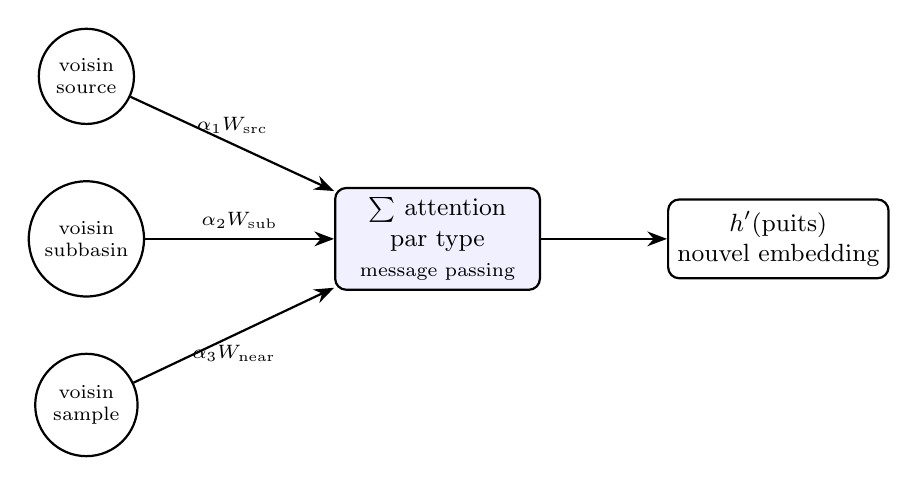
\begin{tikzpicture}[node distance=0.7cm and 1.6cm]
  \node[node_t] (v1) {voisin\\ source};
  \node[node_t, below=of v1] (v2) {voisin\\ subbasin};
  \node[node_t, below=of v2] (v3) {voisin\\ sample};
  \node[stage, right=2.4cm of v2, fill=blue!6] (agg) {$\sum$ attention\\ par type\\{\scriptsize message passing}};
  \node[stage, right=of agg] (h) {$h'(\text{puits})$\\ nouvel embedding};
  \draw[flow] (v1) -- node[above,font=\scriptsize]{$\alpha_1 W_{\text{src}}$} (agg);
  \draw[flow] (v2) -- node[above,font=\scriptsize]{$\alpha_2 W_{\text{sub}}$} (agg);
  \draw[flow] (v3) -- node[below,font=\scriptsize]{$\alpha_3 W_{\text{near}}$} (agg);
  \draw[flow] (agg) -- (h);
\end{tikzpicture}

\end{document}
